%!TEX root = ../memoria.tex

\chapter{Diseño de la solución}

\section{Metodología} \label{sec:Metodologia}



Para desarrollar la plataforma y cumplir con los objetivos planteados en \ref{sec:ObjetivoPrim}, se separó el proyecto utilizando un plan de trabajo que puede resumirse en las siguientes etapas:

\begin{itemize}
\item Analizar algoritmos de reconocimiento acústico para implementar uno de ellos en la plataforma de fiscalización radial, y establecer su configuración según los requerimientos del sistema.

\item Diseñar y desarrollar la plataforma, testeando su funcionamiento con una única radio online, y comprobar que ésta detecta las canciones del repertorio de prueba.

\item Ampliar el alcance de la plataforma para que sea capaz de reconocer canciones de manera simultánea, fiscalizando paralelamente en diversas radioemisoras.
\end{itemize}

\section{Selección de herramientas de desarrollo} \label{sec:SeleccionHerramientas}

En base a la investigación realizada en el apartado \ref{sec:APIS} se establecieron \NumElemTablaComparativaAPIS{} aspectos para comparar los sistemas analizados, y determinar así, cual se ajusta mejor a los requerimientos del proyecto. Por ejemplo, una de las exigencias mas relevantes de la plataforma, según los objetivos secundarios planteados en \ref{sec:ObjetivosSec}, es contar con un base de datos propia que contenga todo el repertorio nacional, incluyendo además, las obras realizadas por artistas independientes, con tal de mantener toda esta información de manera local, ya sea para evitar desfases de tiempo, o cualquier otro tipo de inconveniente, a la hora de ingresar nuevas canciones a la plataforma.

En la tabla \ref{tab:} se señalan las características fundamentales de cada sistema evaluado. De esta colección de herramientas, se ha optado por implementar Dejavu Project, puesto que es la única que establece una conexión local a la hora de analizar y trabajar con los fingerprints. al permitir crear una base de datos propia. De esta forma, el tiempo de búsqueda de coincidencias entre canciones se reduce en comparación a los otros sistemas, si se considera que estos últimos requieren realizar solicitudes a fuentes externas, que no necesariamente estarán actualizadas con los últimos estrenos musicales del país.

\FloatBarrier
\begin{table}[h!]
\centering
\caption{My caption}
\label{tab:CuadroComparativoApis}
\begin{tabular}{lllll}
Elemento             & Dejavu              & bmoquist/ Shazam & bfirsh/ python-echoprint & Music Identification based on Hashed Chroma Features \\
Lenguaje             & Python              & Python           & Python                   & c++                                                  \\
Base de datos        & Local               &                  & Lista en el programa     &                                                      \\
Entrada de datos     & Archivo y micrófono &                  & Lista                    & chroma files of the songs                            \\
Última actualización & Abr-15              & Ene-14           & Nov-12                   & Jul-13                                               \\
Sistema              & Unix-Fedora         &                  &                          &                                                     
\end{tabular}
\end{table}



\subsection{Descripción de Dejavu Project} \label{subsec:DescDejavu}


Como se ha señalado en secciones anteriores, el proyecto Dejavu es un sistema open-source desarrollado en Python, que basa su implementación en fingerprints. Sin embargo, antes de abordar su funcionamiento y especificaciones, en necesario detallar la forma en que la música o señales de audio en nuestro entorno, son transformadas para ser almacenadas en un sistema computacional.



El primer concepto a interiorizar es la aplicación de la Transformada Rápida de Fourier (FFT de sus siglas en inglés: Fast Fourier transform) para el procesamiento digital de señales. Esto debido a que la música es codificada digitalmente como una larga lista numérica. En el caso de un archivo .wav la cantidad de números por canal es del orden de 44100 por segundo, donde los canales corresponden a la secuencia de muestras que un parlante de música puede tocar. Los más habituales son estéreo (2 canales) o mono (un canal). Por tanto, si se contara con una canción promedio de 3 minutos 30 segundos, la cantidad de muestras alcanzaría los:

\begin{equation*}
210 [s]* 44100 \, \bigg[ \frac{muestras}{s} \bigg] *2 \, [canales] = 18.522.000
\end{equation*}

Por su parte, el valor 44100 proviene del teorema de muestreo de Nyquist-Shannon, pero debido al alcance de esta memoria, abordar minuciosamente su descripción no es requerido para comprender el funcionamiento de Dejavu. Basta con señalar que este teorema matemático establece que existe un límite en la frecuencia máxima que es posible capturar con precisión durante la grabación de las señales de audio, y esta frecuencia indica que tan rápido muestreamos la señal, además de establecer que para asegurarse de tomar las muestras necesarias, es requerido aumentar al doble la frecuencia máxima. 



Considerando que el ser humano es incapaz de oír frecuencias por sobre los 20.000 [Hz], la norma establece que un límite de frecuencia máximo es 22.500 [Hz], por lo que utilizando el teorema de Nyquist-Shannon, es posible obtener el valor de las 44.100 muestras por segundo:

\begin{equation*}
Muestras \: por \: segundo = Frecuencia \:  alta * 2 = 22500*2 = 44100.
\end{equation*}

Cabe destacar que en el caso de los archivos .mp3, este formato comprime estos números con la finalidad de ahorrar espacio en el disco.



Una vez se aplica la transforma rápida de Fourier a este conjunto de muestras, es posible generar uno de los elementos más importantes del tratamiento del audio, el espectrograma, una representación visual en dos dimensiones de la amplitud de la señal en función del tiempo y la frecuencia. Como es posible observar de la figura \ref{fig:Angie30Sec}(b), al aplicar la FFT al conjunto de muestras, y unirlas en una sola matriz, se desprende la amplitud de la señal a una frecuencia particular, donde el color rojo corresponde a amplitudes mayores, en oposición al cian, de amplitudes bajas. Vale decir, si se grabara la señal en un solo tono, el espectrograma creado se apreciaría como una línea recta horizontal en la frecuencia de dicho tono.


\begin{figure}[h!]
    \centering
    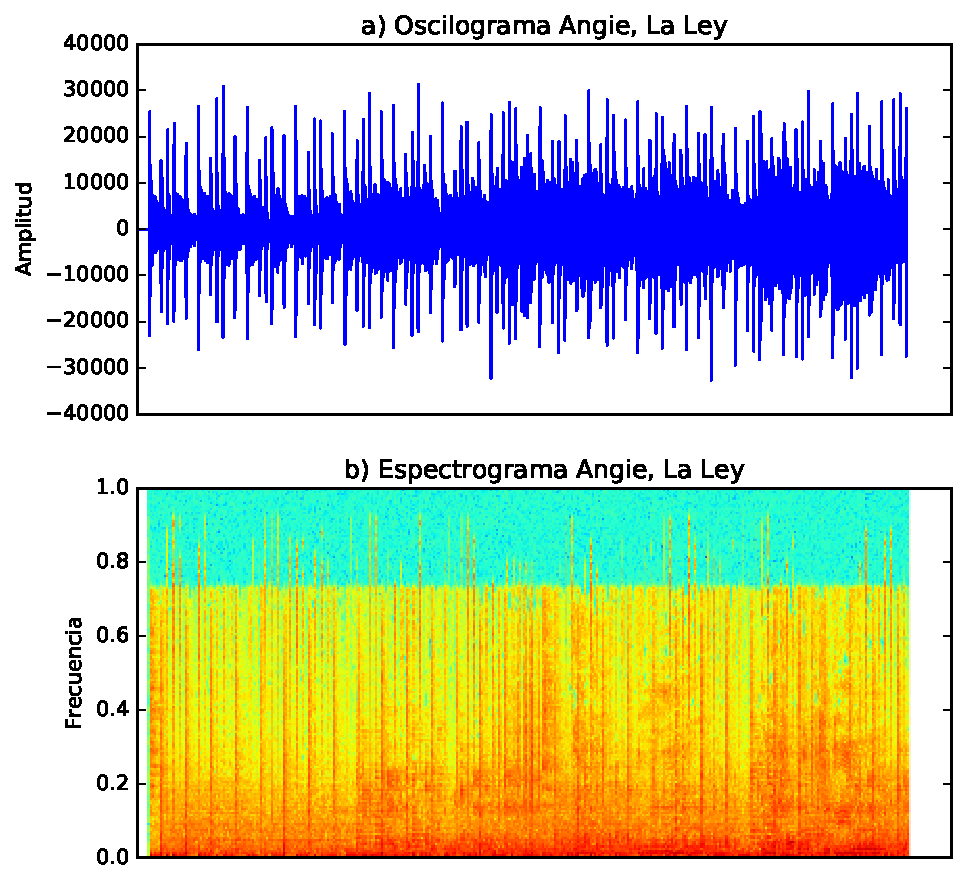
\includegraphics[scale=0.7]{graficos/Angie30Sec.pdf}
    \caption{Modos de representación visual de un archivo de música.}{La figura (a) corresponde a un oscilograma de los primeros 30 segundos de la canción Angie de La Ley que señala la variación de la amplitud respecto al tiempo. La imagen (b) es la representación gráfica de la misma canción, llamada espectrograma, donde la variable dependiente es la frecuencia, en función del tiempo.}
    \label{fig:Angie30Sec}
\end{figure}

Ahora, si bien cabe esperar que este espectrograma sea único para cada canción o audio, se debe tener en consideración que cualquier tipo de ruido que afecte las muestras de grabaciones en el ambiente donde se reproduce la música, provocará que la representación matricial por espectrogramas varíe una infinidad de veces, dependiendo del tipo de ruidos externos que se filtren en la grabación. Por tanto, para los algoritmos de reconocimiento acústico, es necesario encontrar la forma de identificar huellas únicas para cada canción, independiente del ruido que exista en los archivos de audio.

Una forma de hacerlo, es centrándose en las amplitudes más grandes de una canción, pues debido a sus altos valores, no son afectados por posibles ruidos que pueda contener el archivo de entrada. De esta forma, se definen peaks de audio, correspondientes al par de variables tiempo y frecuencia, que aluden a alguna amplitud cuyo valor es el más alto dentro de un vecindario de muestras, de tal forma que es posible discretizar la señal de audio en valores enteros, a partir de las amplitudes más grandes.

Para lograr lo anterior, Dejavu utiliza las herramientas de la biblioteca scipy para tratar el audio de entrada e identificar los máximos locales, tal como lo señala la imagen \ref{fig:EspectrogramasDePeaks}.b . De este modo, se extrae toda aquella información del espectrograma que represente amplitudes altas, por lo que, para cierto margen, el ruido de un archivo ya no influye en el algoritmo.

No obstante, es posible que más de algún par discreto de [tiempo, frecuencia] de alta amplitud en una canción, coincida con pares provenientes de otras canciones, por lo que es necesario volver a tratar la información obtenida. En base a esto, surge otro concepto relevante del procesamiento de música, los fingerprints, o huella digital acústica. Ésta se define como el resumen generado a partir de una señal de audio, que contempla la utilización de una función hash, para crear, a partir de una entrada, una salida alfanumérica que representa la información que le fue dada inicialmente. Por lo tanto, los datos de entrada generan una cadena que solo pueden crearse con esos mismos datos.

\begin{figure}[h!]
    \centering
    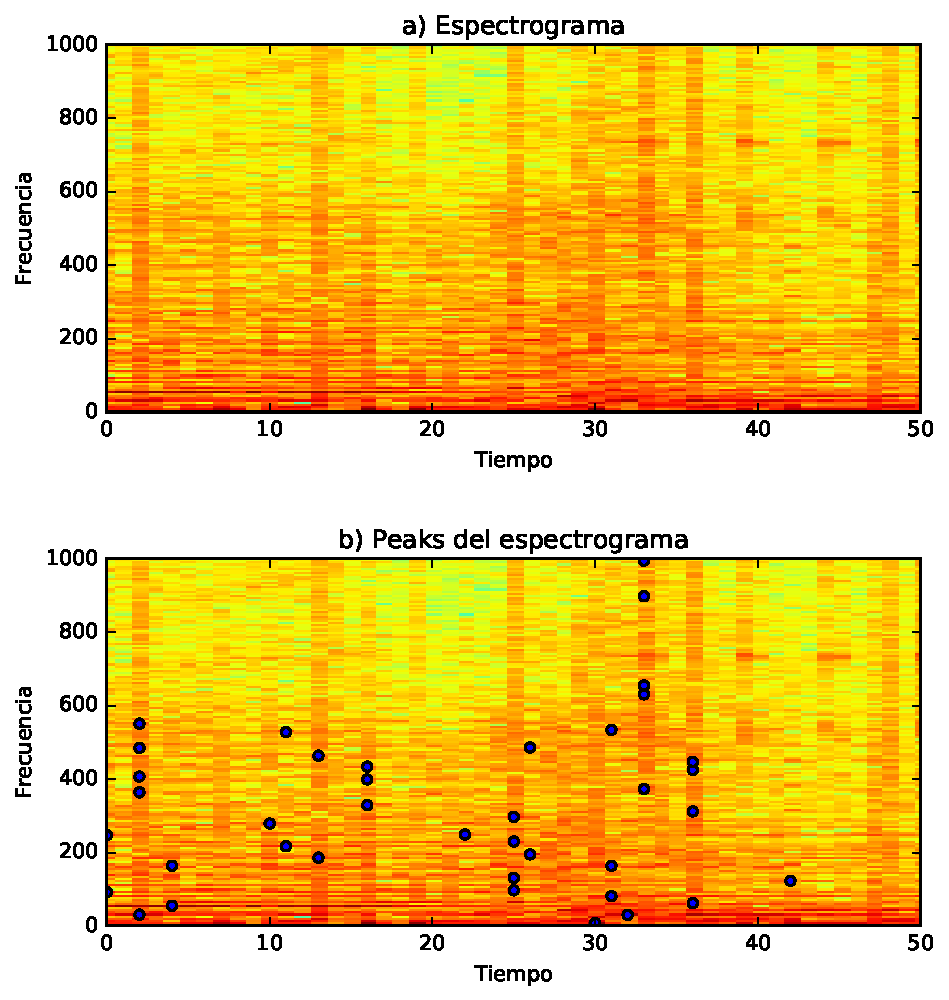
\includegraphics[scale=0.7]{graficos/EspectrogramasDePeaks.pdf}
    \caption{Espectrograma con sus peaks de audio.}{La imagen (a) corresponde a una porción aumentada del espectrograma de los primeros 30 segundos de la canción Angie de La Ley. En (b) se observa el mismo espectrograma con los peaks de audio, cuyos valores de tiempo-frecuencia son utilizados para la creación de fingerprints.}
    \label{fig:EspectrogramasDePeaks}
\end{figure}


Específicamente, la información resumida que contempla un fingerprint corresponde una combinación entre el valor de la frecuencia en un peak del audio, y la diferencia en tiempo, entre algún peak aledaño dentro del vecindario, como se observa en la figura \ref{fig:LineasDePeaks}. Específicamente, Dejavu …[revisar código fuente]. De tal forma que al combinar estos peaks en función del tiempo que los separa, es posible identificar elementos en el archivo que son únicos para cada canción.

\begin{figure}[h!]
    \centering
    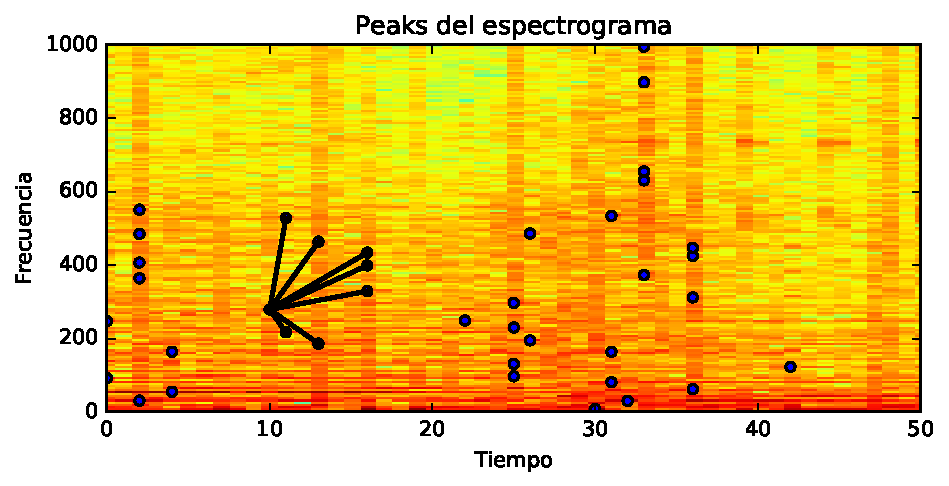
\includegraphics[scale=0.7]{graficos/LineasDePeaks.pdf}
    \caption{Espectrograma con sus peaks de audio.}{La imagen (a) corresponde a una porción aumentada del espectrograma de los primeros 30 segundos de la canción Angie de La Ley. En (b) se observa el mismo espectrograma con los peaks de audio, cuyos valores de tiempo-frecuencia son utilizados para la creación de fingerprints.}
    \label{fig:LineasDePeaks}
\end{figure}

Una vez comprendido los conceptos básicos que permiten caracterizar a cada una de las canciones, creando perfiles únicos para su identificación, es posible abordar el funcionamiento de Dejavu. En primer lugar, se debe contar con un sistema que permita almacenar los diversos fingerprints en una base de datos, puesto que ésta será utilizada para comparar sus registros, con el extracto de canción que se desea reconocer.



La base de datos utilizada con Dejavu es MySQL, cuyo esquema contiene solo dos tablas, fingerprints y songs, con una clave foránea \textbf{song\_id} autoincremental que las relaciona.

\FloatBarrier
\begin{table}[h!]
\centering
\caption{Nombre y tipos de datos que conforman las tablas de la base de datos de Dejavu.}
\label{tab:TablasDejavu}
\begin{tabular}{@{}cll@{}}
\toprule
\midrule
Tabla                         & \multicolumn{1}{c}{Dato} & \multicolumn{1}{c}{Tipo} \\ \midrule
\multirow{3}{*}{songs \vspace{1em}}        & song\_id                 & mediumint unsigned       \\
                              & song\_name               & varchar(250)             \\ \midrule
                              & fingerprinted            & tinyint                  \\
\multirow{3}{*}{fingerprints \vspace{1em}} & hash                     & binary(10)               \\
                              & song\_id                 & mediumint unsigned       \\
                              & offset                   & int unsigned             \\ \midrule \bottomrule 
\end{tabular}
\end{table}


Teniendo en consideración que se crean muchos fingerprints por canción, el campo hash es un binary(10) con tal de reducir el espacio en la base de datos.

...


Se deben mencionar, además, los archivos .py que componen a Dejavu project. \textbf{\_init\_.py} contiene las definciones de la clase Dejavu cuyos métodos más relevantes son \textbf{get\_fingerprinted\_songs} puesto que informa si existe o no una determinada canción en la base de datos y así evitar información redundante. Y en segundo lugar se encuentra \textbf{recognize}, encargada de llamar a los módulos que se dedican a generar los fingerprints de el extracto de una canción, y así comenzar la búsqueda en la base de datos para el posible reconocimiento.

A su vez, \textbf{database.py} y \textbf{database\_sql.py} contienen las funciones que se encargan de implementar y manejar la base de datos. El primer archivos solo contiene el nombre de los métodos, como mera referencia para la ejecución del mismo. Mientras que la segunda detallas las definiciones del archivo anterior, donde se incluye la configuración de la conexión con la base de datos, y toda consulta utilizada por las diversas secciones de Dejavu, como creación de tablas y función hashing.

El par de archivos \textbf{decoder.py} y \textbf{wavio.py} contienen las funciones que permiten el procesamiento de la música. El primero hace uso de Pydub, una librería de python desarrollada para la manipulación de archivos de audio, de tal forma que, a la hora de ingresar canciones al sistema, basta con proporcionarle al objeto Dejavu el directorio que contiene los archivos .mp3 o .wav para que comience el proceso de identificación y generación de fingerprints. No obstante, Pydub no soporta arhivos .wav de 24-bit, por lo que en dicha instancia, llama a \textbf{wavio.py}
 
Un sexto archivo es \textbf{fingerprint.py}, cuya finalidad es el análisis de los arhivos de audio para reconocer los peaks de las canciones, y por consiguiente, de la generación de fingerprints, mediante su método \textbf{get\_2D\_peaks}. También, incluye el método \textbf{generate\_hashes}, que como lo indica su nombre, provee de la estructura para la generación del índice hash. Se debe agregar que dicho archivo también contiene 5 variables que pueden ser modificadas a la hora de ejecutar el programa, pues sus valores permiten variar la cantidad de fingerprints, a costa de disminuir la calidad de las solución entregada por el sistema, y con ello, la seguridad de la respuesta. Estas variables son: \textbf{DEFAULT\_OVERLAP\_RATIO}, \textbf{DEFAULT\_FAN\_VALUE}, \textbf{DEFAULT\_AMP\_MIN}, \textbf{PEAK\_NEIGHBORHOOD\_SIZE}, y \textbf{PEAK\_SORT}.
 
Y para finalizar, existe \textbf{recognize.py}, que como se mencionó en párrafos anteriores, es un módulo llamado desde \textbf{\_init\_.py}. Éste contiene dos clases cuya funcionalidad es muy similar. La clase \textbf{FileRecognizer} utiliza un archivo de audio para comenzar el reconocimiento acústico, mientras que la clase \textbf{MicrophoneRecognizer}, permite utilizar el micrófono del dispositivo para realizar el mismo procedimiento, por tanto, su principal diferencia es el tipo de entrada.



\subsubsection{Análisis de funcionalidad}
Una vez escogido el algoritmo de reconocimiento acústico, se procede a realizar pruebas a su funcionamiento, para determinar el comportamiento frente a diversos escenarios que requieren un rendimiento adecuado por parte del programa, de modo de identificar correctamente las canciones.

De esta forma, para evaluar el rendimiento de Dejavu, se han escogido dos circunstancias, que podrían provocar un rendimiento ineficaz por parte del algoritmo. Asimismo, tomando en consideración los atributos del programa mencionados en la sección anterior, se determinará su comportamiento, analizando variables como tiempos de creación de fingerprints y tamaño de la base de datos, además de tiempo de respuesta, aciertos y CONFIDENCIA de las salidas del algoritmo, para determinar la mejor configuración del mismo.

Cabe mencionar, que las características del equipo utilizado para realizar las pruebas mencionadas, se detallan en \ref{sec:CaracDelEquipo}.

\paragraph{A: Tiempo de creación de fingerprints}\label{parrrafoTiempoCreacionF}\mbox{}\\

Utilizando la configuración de Dejavu por defecto, se han creado seis bases de datos, diferenciando cada uno de ellas en la cantidad de canciones, comenzando desde 10 obras musicales hasta 250, con tal de estudiar el tiempo transcurrido para realizar los fingerprints correspondientes.


En la tabla \ref{tab:TiemposOriginales} se comparan las bases de datos creadas, observándose su tamaño, además de tiempos de creación. Se ha elaborado el gráfico de la figura \ref{fig:TiempoFingerprintOriginales}, tomando los valores de ésta, que permite estimar el tiempo que tomaría crear fingerpirnts para 80.000 canciones, al extrapolar con una tendencia lineal. Es importante destacar que el valor 80.000 no es arbitrario, sino que corresponde a una aproximación realizada por la SCD sobre la actividad musical del país \cite{NumCanciones80k}.


\begin{figure}[h!]
    \centering
    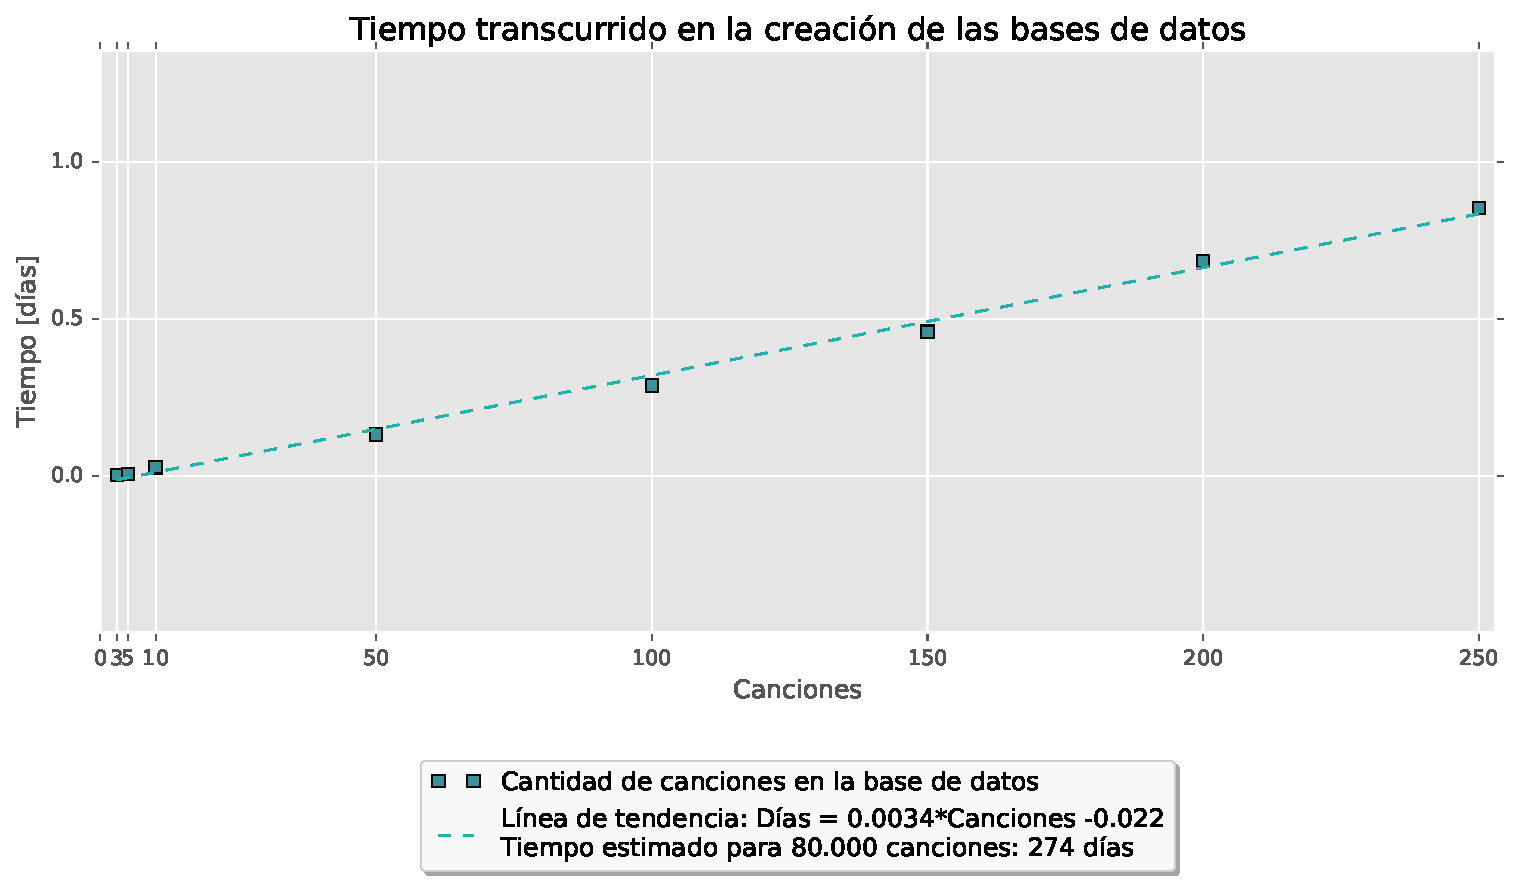
\includegraphics[scale=0.6]{graficos/TiempoFingerprintOriginales.pdf}
    \caption{Tiempo en función del número de canciones con la configuración original de Dejavu.}{La ecuación de la línea de tendencia, permite extrapolar el valor de los días necesarios para crear la base de datos de 80.000 canciones de la plataforma.}
    \label{fig:TiempoFingerprintOriginales}
\end{figure}


Analizando la ecuación del gráfico se obtiene un tiempo de 274 días, por lo que se hace necesario modificar los atributos originales del programa para reducir el tiempo de creación de la base de datos oficial de la plataforma.

\paragraph{B: Análisis de atributos de configuración}\label{parrrafoAnalisisAtributos}\mbox{}\\

Según lo descrito en \ref{subsec:DescDejavu}, Dejavu cuenta con cinco atributos que pueden ser modificado a la hora de crear la base de datos, por lo que cada uno de ellos fue analizado por separado. Las bases de datos contienen las mismas canciones, pero que cuya cantidad varía entre  3 y 5, con tal de identificar la forma en que cada elemento analizado influye en el número de fingerprints creados.

La tabla \ref{tab:ConfiguracionBDD35} del apéndice contiene los valores de configuración de cada base de datos diseñada, con sus respectivos tiempos de creación, tamaños y cantidad de fingerprints. Estos datos se utilizan para la generación de los gráficos de la figura \ref{fig:FingerprintsEnFuncionVariables} que permitan identificar la relación entre cada uno de estos parámetros, con su respectiva cantidad de fingerprints. Las variables DEFAULT\_OVERLAP\_RATIO y DEFAULT\_FAN\_VALUE son curvas crecientes, por lo que el aumento de fingerpirnts es proporcional al aumento en el valor del parámetro. En tanto, DEFAULT\_AMP\_MIN y PEAK\_NEIGHBORHOOD\_SIZE tienen comportamiento inverso. Hay que mencionar además, que la quinta variable estudiada, llamada PEAK\_SORT, es una variable booleana, que al modificarle el valor a \textbf{False}, la cantidad de fingerprints desciende considerablemente en comparación a las otras bases de datos. No obstante, no se realizaron mayores estudios de dicha variable debido al mal rendimiento que ocasiona esta disminución en el número de identificadores únicos de cada canción.

\begin{figure}[h!]
    \centering
    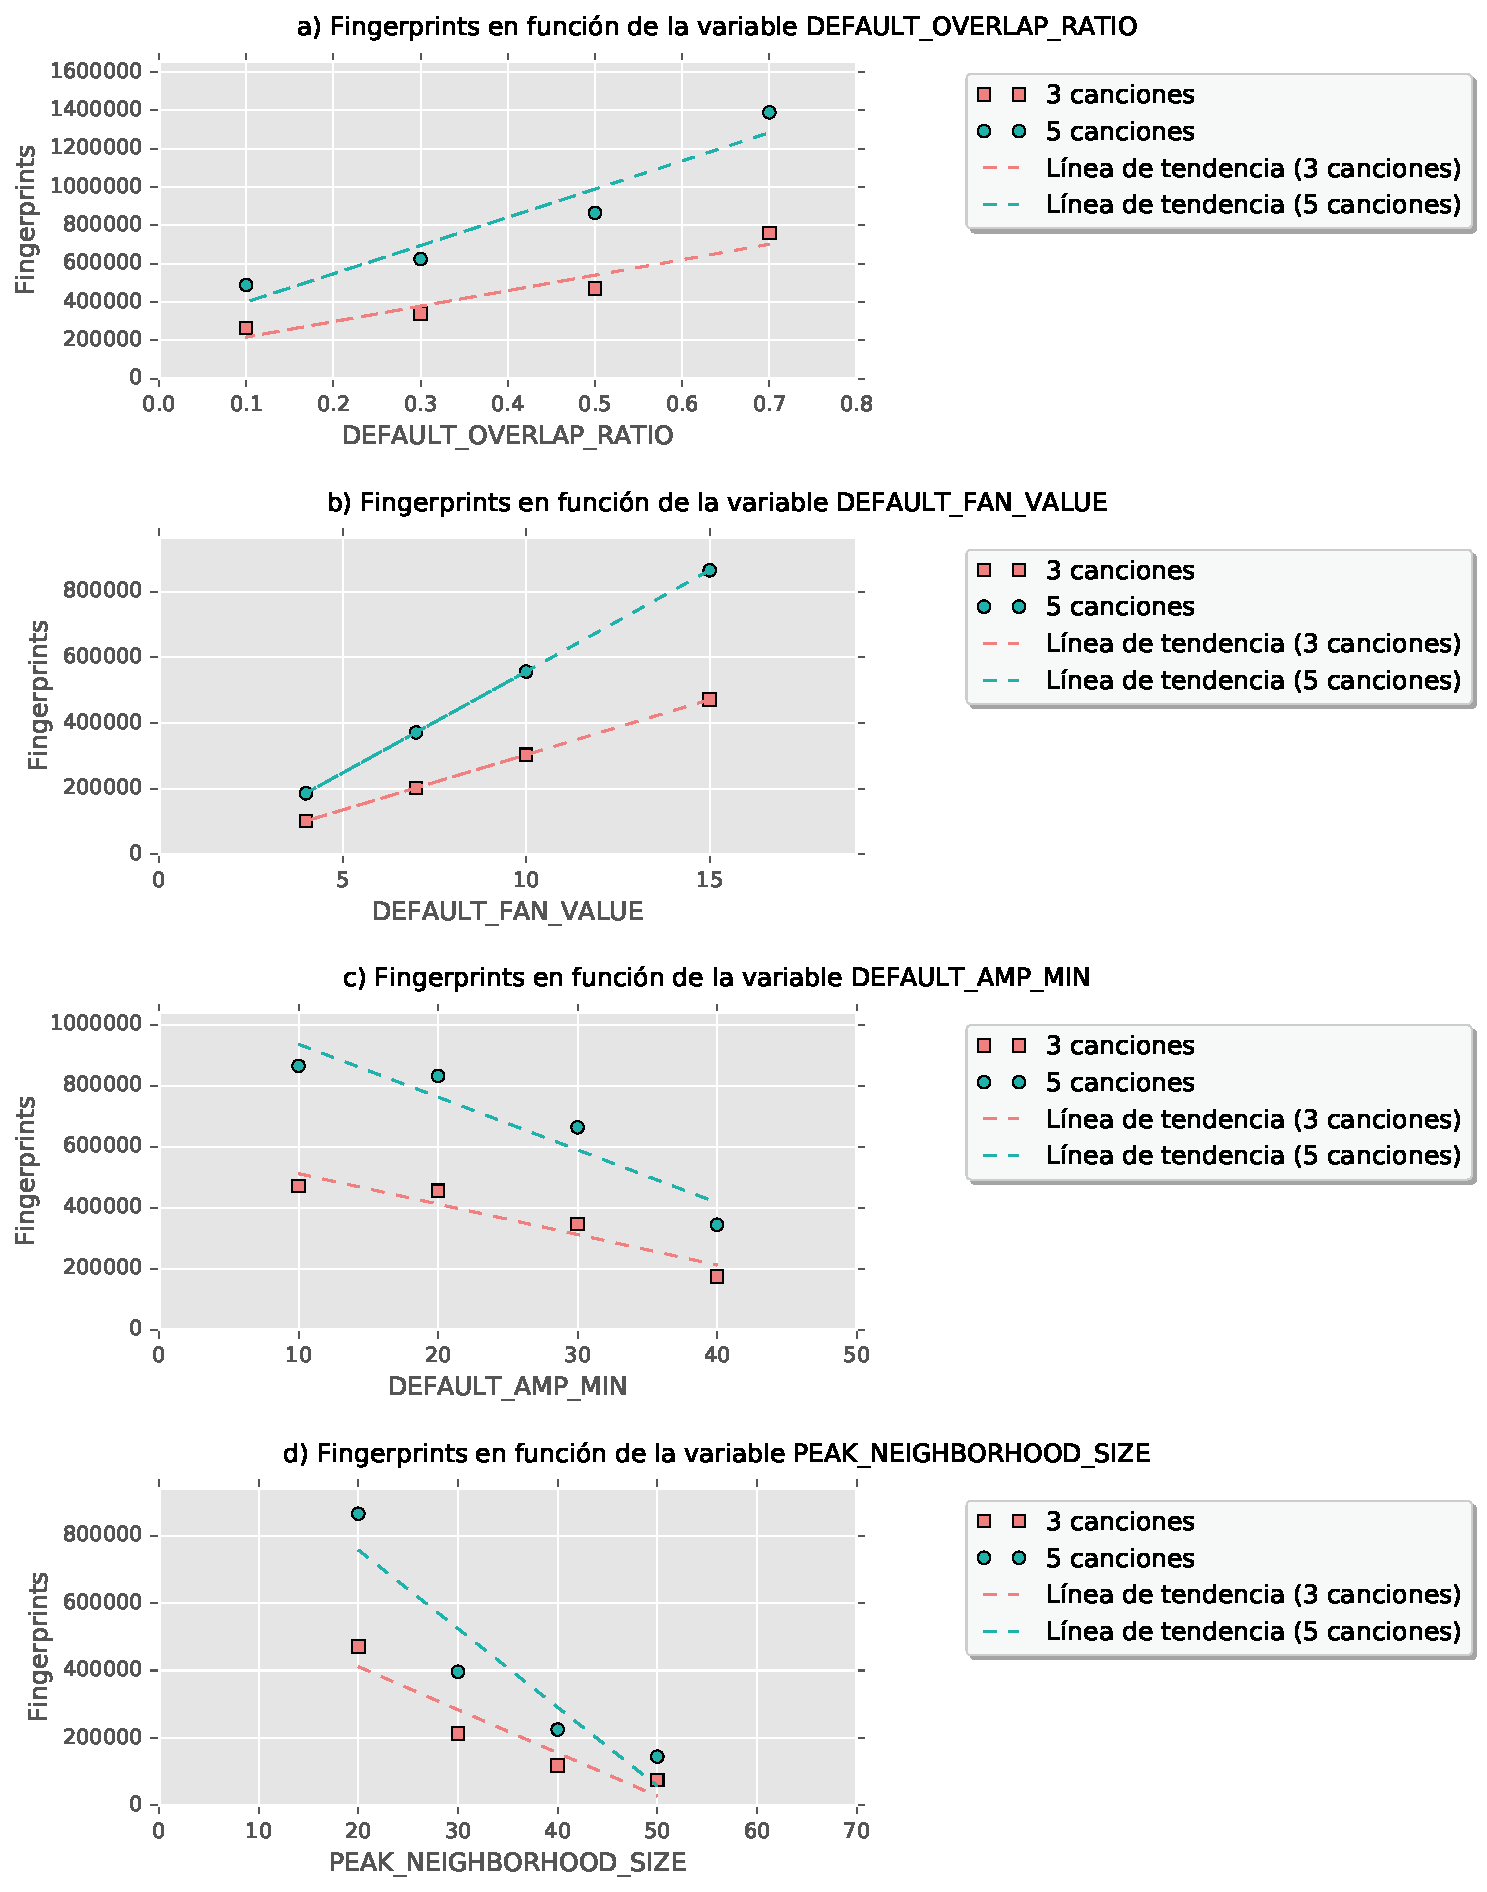
\includegraphics[scale=0.6]{graficos/FingerprintsEnFuncionVariables.pdf}
    \caption{Fingerprints en función de diversos valores de configuración.}{Los gráficos muestran la variación de la cantidad de fingerprints en función de los valores asignados a las variables de configuración: DEFAULT\_OVERLAP\_RATIO y DEFAULT\_FAN\_VALUE como rectas crecientes, PEAK\_NEIGHBORHOOD\_SIZE y DEFAULT\_AMP\_MIN como rectas decrecientes.}      
    \label{fig:FingerprintsEnFuncionVariables}
\end{figure}

Una vez creadas las bases de datos, se consideraron los siguientes factores para analizar el algoritmo de Dejavu, realizando pruebas de reconocimiento acústico:

\begin{itemize}
\item Tiempo de respuesta de Dejavu: indica el lapso que transcurre desde que el algoritmo recibe una consulta, crea los fingerpirnts del extracto de música analizado, y se buscan coincidencias en la base de datos, hasta que se devuelve la respuesta.

\item Confianza: determina el porcentaje de veracidad o certeza de la respuesta entregada por el algoritmo.

\item Acierto: esta variable determina efectivamente si la salida del algoritmo corresponde al extracto de canción analizado.

\item Tamaño del extracto: elemento medido en segundos que determina la duración de cada archivo de música de prueba, abarcando un rango de 5, 10 y 15 segundos.

\item Sección del extracto: corresponde al momento en que se ha creado un extracto de música de prueba. De esta forma, se comprueba si el algoritmo acierta con la respuesta, independiente si la solicitud de reconocimiento acústico se hizo al principio, al final, o en la mitad de la canción. 
\end{itemize}

Para realizar las pruebas, se escogieron tres canciones presentes en todas las bases de datos diseñadas, y se crearon extractos de 5, 10 y 15 segundos de cada una de ellas. La extensa salida de los resultados fue resumida en la tabla \ref{tab:Resumen3Canciones} del apéndice, que en conjunto con los gráficos de la figura \ref{fig:AnalisisTest35Canciones}, permiten extrapolar el tiempo necesario para la plataforma de 80.000 canciones. 

La primera afirmación que se puede realizar es la relación proporcional entre la cantidad de segundos del extracto de música que Dejavu analiza, con la cantidad de aciertos, pues a medida que aumentan los segundos, también lo hace las respuestas correctas entregadas por Dejavu. Es más, para extractos de 15 segundos, la mayoría de las respuestas son consideradas correctas. A partir de esta observación, se establece que para el algoritmo de la plataforma, se utilizarán extractos de esta cantidad de segundos para analizar el streaming de las radios.

Además, a simple vista se observa que la base de datos E1, aquella que modifica PEAK\_SORT como valor \textbf{False}, redujo en mayor proporción el numero de fingerprits creados, por lo que su tiempo estimado es el menor de todos. Empero, tuvo un improductivo rendimiento, donde solo logró 3 aciertos cuando se utilizaba un extarcto de 15 segundos, y en consecuencia, el valor de este booleano no es considerado como posible factor para la configuración de Dejavu, puesto que la limitada cantidad de fingerprints reduce el desempeño del algoritmo de reconocimiento acústico.

Teniendo en cuenta que, la razón para modificar los valores de configuración, es reducir el tiempo de la creación de la base de datos, se preseleccionan las bases B1, B2 y B3 debido a sus reducidos tiempos estimados en días, para la creación de la base de datos. Además presentan un buen rendimiento, al revisar el número de aciertos por el total de pruebas realizadas, siendo solo 1 de 9, de los extractos de 5 segundos el que obtuvo una respuesta incorrecta. 

\paragraph{C: Prueba de extractos de música inexistentes en la base de datos}\label{parrrafoPrubasNoMusica}\mbox{}\\

Una segunda característica esencial, esperable de un buen rendimiento , además del número de aciertos, es el comportamiento del algoritmo en las ocasiones en que la canción testeada no es parte del repertorio.

Dado que la idea fundamental de esta plataforma es albergar solo la música chilena, se hizo este análisis con el propósito de determinar como sería mayoritariamente el comportamiento del algoritmo, debido a que, en general, la programación emitida por las radioemisoras nacionales es extranjera, y por consiguiente, la mayoría de la parilla radial emitida en el país, no será almacenada en la plataforma.

Por estas razones, se realizaron las mismas pruebas de reconocimiento acústico que en el caso anterior, con la salvedad que, a Dejavu se le asignó de entrada, archivos de música que no existen en la base de datos. Los resultados de la tabla \ref{tab:Resumen3SinCanciones} señalan que las tres configuraciones preseleccionadas, B1, B2 y B3, no obtuvieron el resultado esperado. Es más, para todas las pruebas realizadas, Dejavu efectivamente devolvió un listado con el nombre de diversas canciones, sin embargo, estas respuestas eran erróneas, pues lo correcto hubiese sido que el algoritmo devolviera un valor nulo para cada una de ellas, pues las canciones no existían en las base de datos analizadas.

Para ahondar en el estudio de este comportamiento, se analiza la fila de confianza máxima de las respuesta erróneas y confianza mínima de los aciertos de las tablas de resultados, pues así, es posible establecer un delta que permita definir un límite para aquellas respuestas erradas entregas por Dejavu. Vale decir que, independientemente que Dejavu devuelva el nombre de alguna canción, éste puede ser incorrecto, por tanto, si la confianza de esta respuesta no supera cierto umbral, no se considera segura.

De la tabla \ref{tab:Resumen3Canciones} donde sí hay respuestas correctas, el valor mínimo de confianza de los aciertos es de 68, 126 y 179 para B1, B2 y B3 respectivamente. Mientras que de la tabla \ref{tab:Resumen3SinCanciones} se desprenden que la confianza máxima de los errores es de 4 para cada base de datos preseleccionada. Debido a este bajo valor, es esperable que el nombre de la canción devuelto por Dejavu sea incorrecto. Como resultado, las respuestas con valores de confianza que se encuentren dentro de este delta, deben ser fácilmente identificadas a la hora de fiscalizar y realizar el listado de canciones emitidas por una radio, puesto que lo más seguro es que el nombre no sea correcto. 

Dentro de este marco, al entrecruzar toda la información de tablas y gráficos presentados en este capítulo, revisando además el número de aciertos, en conjunto con los valores de tiempo estimado para creación de la plataforma, se ha optado por B2 como la configuración final de Dejavu, cuyos parámetros se definen en la tabla \ref{tab:NuevaConfiguracionBDD}


\FloatBarrier
\begin{table}[h!]
\centering
\caption{Valores de los parámetros de la nueva configuración de Dejavu.}
\label{tab:NuevaConfiguracionBDD}
\begin{tabular}{@{}lr@{}}
\toprule
\midrule
\multicolumn{1}{c}{Parámetro} & \multicolumn{1}{c}{Valor}  \\ \midrule
DEFAULT\_OVERLAP\_RATIO   & 0,5                       \\
DEFAULT\_FAN\_VALUE       & 7                        \\
DEFAULT\_AMP\_MIN         & 10                        \\
PEAK\_NEIGHBORHOOD\_SIZE  & 20                        \\
PEAK\_SORT                & True                      \\ \midrule \bottomrule
\end{tabular}
\end{table}



\paragraph{Prueba de covers en Dejavu}\label{parrrafoPruebasCovers}\mbox{}\\

A continuación, es necesario examinar un último escenario, que consiste en evaluar el comportamiento de Dejavu, sobre aquellas canciones de artistas que han sido interpretadas por otro músicos, creando nuevas versiones de una obra musical.


Es esperable que los fingerprints entre covers tengan cierta similitud debido a la semejanza de sus ritmos musicales, por lo que se ha escogido una serie de canciones para observar las respuestas del algoritmo. Inicialmente se escogieron canciones disponibles en la base de datos, y luego, se eliminaron algunas para comprobar si la respuesta de Dejavu sería o no el cover correspondiente.

Resultados...


\section{Descripción del programa} \label{sec:DescripcionPrograma}

\subsection{Fiscalización de una radioemisora online}

De acuerdo a la metodología implementada, tras escoger y configurar el algoritmo de reconocimiento acústico para el programa de fiscalización, se procede a desarrollar la plataforma, de tal forma que abarque solo la supervisión de una única radio online. Por tanto, para abordar este requerimiento, se identificaron las tareas fundamentales del sistema para lograr su funcionamiento, las que se aprecian en el siguiente seudocódigo.




\begin{algorithm}
\begin{algorithmic}[1]
\REQUIRE \textit{urlRadio, nombreRadio, segundosExtracto, fechaLimite, delay.}
\ENSURE archivo de texto plano.
\STATE craerArchivoSalida(nombreRadio)
\WHILE {(tiempo actual $<$ \textit{fechaLimite})}
\STATE Acceder a \textit{urlRadio} del streaming
\STATE Transformar señal continua de música en discreta creando extractos de \textit{segundosExtracto} 
\STATE Reconocer extracto de música con Dejavu
\STATE Exportar respuesta a documento de fiscalización
\ENDWHILE

\end{algorithmic}
\caption{Fiscalización de una radioemisora online}\label{alg:Fiscalizacion1Radio}
\end{algorithm}

En líneas generales, el programa requiere estar constantemente accediendo a la url del streaming, cada cierto intervalo de tiempo, con tal de generar múltiples archivo de música, los que serán transmitidos a la función de Dejavu que se encarga del reconocimiento acústico. De este modo, es posible generar una lista de las canciones que están siendo emitidas en una determinada radio online.  

\begin{framed}

Agregar requerimientos: conexión a internet. URL streaming.

\end{framed}

El detalle de las variables de entrada del programa se presenta a continuación:

\begin{itemize}
\item \textit{urlRadio}: cadena que almacena el link del streaming de la radio que se controla.
\item \textit{nombreRadio}: variable que identifica por un nombre corto la radio que se analiza, y cuyo valor será utilizado para nombrar el archivo de salida.
\item \textit{segundosExtracto}: variable entera que indica la duración que tendrán los extractos de música creados desde el streaming.
\item \textit{fechaLimite}: variable tipo fecha que puede ser definida de dos formas.
\begin{itemize}
\item fechaLimite en minutos: esta variable contabiliza el tiempo desde que se corre el programa hasta que transcurran los minutos definidos por el usuario.
\item fechaLimite como día: el programa se ejecuta hasta el día, hora, minutos y segundos, que se le definieron.
\end{itemize}
\item \textit{delay}: variable entera definida en segundos, que indica cada cuanto tiempo se están creando extractos de música desde la radio, para transformar la señal continua en discreta, y hacer uso de Dejavu para su reconocimiento.
\end{itemize}

Cabe mencionar que la salida del programa corresponde a un archivo de texto, el cual es creado a partir del método \textit{craerArchivoSalida(nombreRadio)}. Éste contiene el listado del nombre de las canciones, con sus respectivos tiempos cronológicos de emisió., 

Para el ciclo iterativo (líneas 2 a 7) se desarrolló una función nombrada \textit{fiscalizar}, la que se llama a sí misma cada cierto tiempo definido por la variable \textit{delay}, hasta que se ha alcanzado el tiempo de fiscalización indicado por \textit{fechaLimite}. La función \textit{fiscalizar}, a su vez, llama a la función \textit{generarExtracto}, pero en un nuevo hilo de ejecución. De esta forma, independiente que el algoritmo tarde mucho en reconocer alguna canción, seguirán creándose extractos según los segundos definidos, sin necesidad de esperar la respuesta de Dejavu para seguir con la ejecución del programa.


\textit{generarExtracto} por su parte, corresponde a la función con más líneas de código, debido a que agrupa las tareas fundamentales del programa. El próximo seudocódigo especifica su labor.

\begin{algorithm}
\begin{algorithmic}[1]
\REQUIRE \textit{urlRadio, nombreRadio, segundosExtracto, fechaLimite, delay.}
\STATE Determinar \textit{nombreArchivo} del extracto de música de extensión .mp3 que se creará desde el streaming
\STATE Conexión streaming \textit{urlRadio}
\WHILE {(segundos transcurridos $<$ \textit{segundosExtracto*2})}
\STATE crear extracto \textit{nombreArchivo}.mp3
\ENDWHILE 
\STATE \textit{cortarCancion(nombreArchivo, segundosExtracto)}
\STATE cancion $=$ dejavu.recognize(\textit{nombreArchivo})
\STATE \textit{contenidoFila} = generar cadena texto para imprimir en archivo de salida, incluyendo nombre de la canción reconocida, fecha en que sonaba, y tiempo de respuesta de dejavu
\STATE \textit{actualizarArchivoSalida(contenidoFila)}

\end{algorithmic}
\caption{generarExtracto}\label{alg:GenerarExtracto}
\end{algorithm}



Con respecto a la tercera línea de código del Algoritmo \ref{alg:GenerarExtracto} es importante destacar que el valor de la variable \textit{segundosExtracto} es duplicado, debido a que la duración real de la extracción de audio desde el streaming, varía en función de la memoria, tiempo de respuesta del servidor del streaming, etc, por lo que en caso de no aumentar su extensión, estos archivos serán más cortos que el tiempo requerido. Por tanto, \textit{cortarCancion} de la línea de código 6 es una función que se encarga de modificar la duración del archivo de música descargado, según los parámetros definidos por el usuario.

Como se especifica en la cuarta línea de código, se crean archivos de audio de extensión .mp3 que contienen los extractos de música obtenidos desde la url del streaming de la radio, debido a que es el tipo de archivo que requiere como parámetro la función de reconocimiento acústico de Dejavu, y por ello, se hace indispensable transformar la señal continua de música en pequeños extractos. A su vez, el nombre de estos archivos contienen información sobre la fecha en la que fueron creados, por lo que será posible realizar una planilla que contenga la parilla musical de la radio fiscalizada, una vez el extracto de música sea reconocido por el algoritmo. Así, en la línea 7 del código, se define la variable \textit{cancion} que almacena la respuesta de Dejavu en formato de diccionario. 

Como resultado, se crea una cadena con todos estos datos, y mediante el método \textit{actualizarArchivoSalida} se imprime en una archivo de texto plano para generar la planilla de la radio, y de esta forma, se registra la música que estaba sonando en un determinado momento. Se debe mencionar, además, que la respuesta de Dejavu puede conducir a tres situaciones. En primera instancia, la música será reconocida, y dicha información será agregada a la planilla, sin embargo, en caso en que el diccionario \textit{cancion} esté vació por no haber coincidencia de fingerprints, o el extracto de música no sobrepasa un umbral de frecuencia y genera un audio vacío, ambas respuestas son claramente señaladas en el archivo de salida, con los respectivos tiempos en que las situaciones recién mencionadas ocurrieron.


\subsection{Fiscalización paralela}
La última etapa del proyecto consiste en probar el algoritmo anterior, modificando los aspectos necesarios para lograr fiscalizar múltiples radioemisoras online a la vez. Cabe destacar que, debido a la forma y estructura en que fue desarrollado el algoritmo anterior, fue sencillo modificar el método \textit{fiscalizar} para generar mayor cantidad de hilos de ejecución y cumplir con el análisis paralelo de las radios.

A continuación se presenta el nuevo algoritmo, indicando las funciones agregadas al desarrollo anterior.


\begin{algorithm}
\begin{algorithmic}[1]
\REQUIRE \textit{archivoEntrada, segundosExtracto, fechaLimite, delay.}
\ENSURE archivos de texto plano con parilla musical.
\STATE listaNombreRadios, listaUrlRadios = \textit{obtenerRadios(archivoEntrada)}
\STATE \textit{crearArchivoSalida(listaNombreRadios)}
\STATE \textit{fiscalizar(listaUrlRadios, listaNombreRadios, segundosExtracto, fechaLimite, delay)}

\end{algorithmic}
\caption{Fiscalización paralela}\label{alg:fiscalizarParalelo}
\end{algorithm}

La primera diferencia es el método \textit{obtenerRadios} el cual se encarga de leer un archivo de entrada de texto plano que contiene el nombre corto de una determinada radioemisora, con su respectiva dirección de streaming. De esta forma, se generan las listas \textit{listaNombreRadios} y \textit{listaUrlRadios}.

Como se mencionó con anterioridad, la función fiscalizar, encargada de generar los extractos y reconocer la música, también fue ligeramente modificada para lograr revisar simultáneamente en varias estaciones de radio online, tal cual lo señala el algoritmo \ref{alg:fiscalizar}.

\begin{algorithm}
\begin{algorithmic}[1]
\REQUIRE \textit{listaUrlRadios, listaNombreRadios, segundosExtracto, fechaLimite, delay.}
\IF {(tiempo actual $<$ \textit{fechaLimite})}
\STATE \textit{inicio} = definir tiempo de inicio
\FOR {(urlRadio \textbf{en} listaUrlRadios)}
\STATE \textit{generarExtracto(urlRadio, nombreRadio, segundosExtracto, fechaLimite, delay)}
\ENDFOR
\STATE \textit{final} = definir tiempo de finalización
\STATE \textit{delayReal} = \textit{delay} - (\textit{final} - \textit{inicio})
\STATE \textit{fiscalizar(listaUrlRadios, listaNombreRadios, segundosExtracto, fechaLimite, delayReal)}
\ELSE
\STATE Detener ejecución
\ENDIF

\end{algorithmic}
\caption{fiscalizar}\label{alg:fiscalizar}
\end{algorithm}
 
De las líneas 3 y 4 del algoritmo \ref{alg:fiscalizar}, se desprende que se generan múltiples llamadas al método \textit{generarExtracto} el cual, al estar dentro de un loop, se encarga de revisar cada radio disponible en el listado \textit{listaUrlRadios}, de tal forma, de crear archivos de música para su posterior identificación, tal como se señala en el método \ref{alg:GenerarExtracto} \textit{generarExtracto} ya definido.

A su vez, el método \textit{fiscalizar} se llama a si mismo una vez a pasado el tiempo de espera definido por \textit{delayReal}. Se ha incluido el cálculo de esta variable debido a que si la generación de múltiples hilos en la ejecución del loop provoca cierto retraso, el tiempo entre el extracto n-ésimo y extracto n+1 de una misma radio, mantendrá el \textit{delay} original definido, sin considerar el tiempo utilizado para la generación de extractos de las otras radios.

Para finalizar, se debe recordar que la función \textit{actualizarArchivoSalida} del algoritmo \label{alg:GenerarExtracto} es la encargada de imprimir en un archivo de texto el listado de las canciones reconocidas con dejavu, con sus respectivos tiempos, de tal forma de generar automáticamente múltiples archivos con la parilla musical del listado de radios online.





